\documentclass[a4paper,titlepage]{article}

% use this when images are included
\usepackage{float}
\usepackage{graphicx}
\graphicspath{ {./images/} }

% use for lines of code
\usepackage{listings}

% use for links, also links list of contents
\usepackage{hyperref}

\usepackage[
    top    = 2.75cm,
    bottom = 2.50cm,
    left   = 3.00cm,
    right  = 2.50cm]{geometry}

\begin{document}
\thispagestyle{empty}

\section*{Varroa Destructor Destructor or The Un-Mite-y Bee\\- Saving our friendly honey makers}

\begin{figure}[H]
    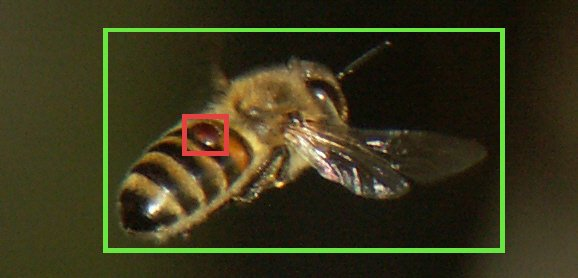
\includegraphics[width=\textwidth]{Biene_mit_Varroa_erkannt.jpg}
\end{figure}

\section*{The German Mite Busters}

\subsection*{Max-Felix Müller}
\begin{tabular}{rl}
\textsc{E-Mail:} & mxfxmmueller@gmail.com \\
\textsc{Credentials:} & Electrical Engineer - Embedded Software \\
\textsc & Pancake detector based on OpenCV \\
\textsc & Bottle classification using Jetson Nano \\
\textsc & Electric Wheelbarrow
\end{tabular}

\subsection*{Frank Münzner}
\begin{tabular}{rl}
\textsc{E-Mail:} & frank.muenzner@fpem.de \\
\textsc{Credentials:} & Electrical Engineer - Microsystems \\
\textsc & Premature failure analysis using OpenCV \\
\textsc & Object detection on Jetson Nano / Xavier \\
\textsc & Image detection and processing on LabView
\end{tabular}

\subsection*{Adam Müller}
\begin{tabular}{rl}
\textsc{E-Mail:} & adtheomueller@gmx.de \\
\textsc{Credentials:} & Mechatronics Engineer - Robotics \\
\textsc & 6-Axis Robot Arm \\
\textsc & Formula Student HHN - Head of Electronics
\end{tabular}

\subsection*{Lukas Dietz}
\begin{tabular}{rl}
\textsc{E-Mail:} & lukas.dietz@online.de \\
\textsc{Credentials:} & Software Engineer \\
\textsc & Formula Student Highspeed Karlsruhe - Head of Electronics \\
\textsc & X-Box CPU Modding
\end{tabular}

\newpage
\thispagestyle{empty}
\section*{Description}

The honey bee belongs to the class of insects, pollenising plants and therefor playing a significant role in nature not only in the survival of different types of plants but also as a basic requirement of our food supply.
In the last decade a considerable decline in honey bee population was observed.
There are many hypotheses about the possible causes.
Besides the use of insecticides, a major reason for bee mortality is the weakening of bee colonies by parasites.
The best known parasite is the varroa destructor.
It is assumed that up to 25\% of bee colonies in Germany do not survive the winter due to the infestation and the associated weakening by the mites. 

The varroa destructor is a parasitic mite, feeding on honey bees.
Furthermore, the mite carries bacteria and viruses into the bee colony.
The mite is about $ 2 mm^2 $ in size and attacks the bee by attaching to them and sucking the bees fat body.
The varroa mite lays eggs on the bee larva.
An infestation harms not only the bees directly affected, but may also lead to the death of the whole colony.

Currently there is no easy way to continuously monitor levels of varroa mites.
Some methods either harm or kill the bees, at least those used as a sample, or take a long time to get a result.
A possible method to get a continuous and timely overview of the size of the Varroa infestation would be to check the collecting bees flying in and out of the flyway for infestation.

Detecting the mites on the bees using computer vision will be a challenge due to the size alone.
Additionally the mites can attach to the bees not only from the top but also from the bottom, requiring multiple cameras to scan each bee.
We plan on mounting multiple cameras inside each bee hive, collecting as much data as possible.
The timing should be right, since the bees will very soon after the comeptition started also start flying again.

In a very first step, we focus on detecting the bees themselfs.
Counting the number of bees going in an out of the hive already gives insight on the health of the population.
When the classification is working, each bee can then be examined further, checking for pollen yield and the varroa destructor.

Most bee hives are further away from the city, making it difficult to stream images or videos to remote servers.
Using the OAK will enable us to run inference on location.
Only when a bee with the varroa destructor is detected, the owner of the hive will be notified.
He/She can also be notified if any irregularity in the behaviour of the bees is detected.

Reacting early is key in keeping our bees healthy and with the OAK and a suitable software, we can help the bees help us. \\

Thinking one step further, after the detection of the mites and notification of the owner we propose different mehtods of fighting the varroa destructor.

\begin{itemize}
    \item Selective killing of the mites by focused introduction of an active agent, dispatched using for example piezo electric dispensers.
    \item Local heating of the bee or prefferably the mite using a focused laser, either killing the mite directly or making it fall off the bee.
    \item Isolation and/or execution of the infested bee, which can then be trasported out by the worker bees.
\end{itemize}

\section*{Team Info}
\begin{tabular}{rl}
\textsc{Categroy:} & Agriculture \\
\textsc{Region:} & Region 3 \\
\textsc & Europe + Russia + Australasia \\
\textsc & Germany \\
\textsc{Team Type:} & General Team \\
\end{tabular}

\end{document}
